\section{Архитектура}
\subsection{Структура системы}

На основе требований, сформулированных в разделе сбора требований,
была разработана модульная архитектура системы, обеспечивающая
гибкость, расширяемость и возможность проведения воспроизводимых
экспериментов.

Общая структура системы представлена на (рис.~\ref{fig:architecture}).

\begin{figure}[h!]
    \centering
    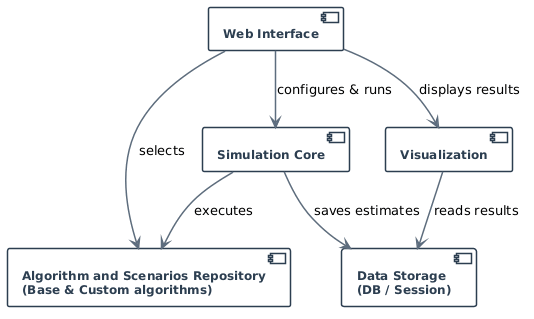
\includegraphics[width=0.9\textwidth]{arch.png}
    \caption{Архитектура системы моделирования}
    \label{fig:architecture}
\end{figure}

Архитектура системы включает следующие основные компоненты:

\begin{itemize}
    \item \textbf{Web Interface (веб-интерфейс).}  
    Обеспечивает взаимодействие пользователя с системой. Через данный
    компонент осуществляется настройка параметров симуляции, выбор
    алгоритмов, запуск экспериментов и просмотр результатов.

    \item \textbf{Simulation Core (ядро моделирования).}  
    Центральный компонент системы, отвечающий за выполнение симуляции,
    генерацию движения целей и обработку наблюдений с учётом шумов.

    \item \textbf{Algorithm Repository (репозиторий алгоритмов).}  
    Содержит базовые и пользовательские алгоритмы и предоставляет
    унифицированный интерфейс для их выполнения.

    \item \textbf{Data Storage (хранилище данных).}  
    Отвечает за сохранение результатов моделирования, параметров
    экспериментов и промежуточных вычислений.

    \item \textbf{Visualization (подсистема визуализации).}  
    Обеспечивает отображение результатов в виде графиков траекторий
    и кривых ошибок.
\end{itemize}

Взаимодействие компонентов (рис.~\ref{fig:architecture}) организовано
следующим образом: пользователь через веб-интерфейс задаёт параметры
симуляции и выбирает алгоритмы, после чего управление передаётся в ядро
моделирования. Ядро обращается к репозиторию алгоритмов, сохраняет
результаты в хранилище и передаёт их в подсистему визуализации.

Таким образом, архитектура удовлетворяет требованиям:
поддержки пользовательских алгоритмов, гибкой настройки,
визуализации и пакетной обработки экспериментов.

\subsection{Пользовательский сценарий}

Типовой пользовательский сценарий работы с системой представлен
на (рис.~\ref{fig:usecase}).

\begin{figure}[h!]
    \centering
    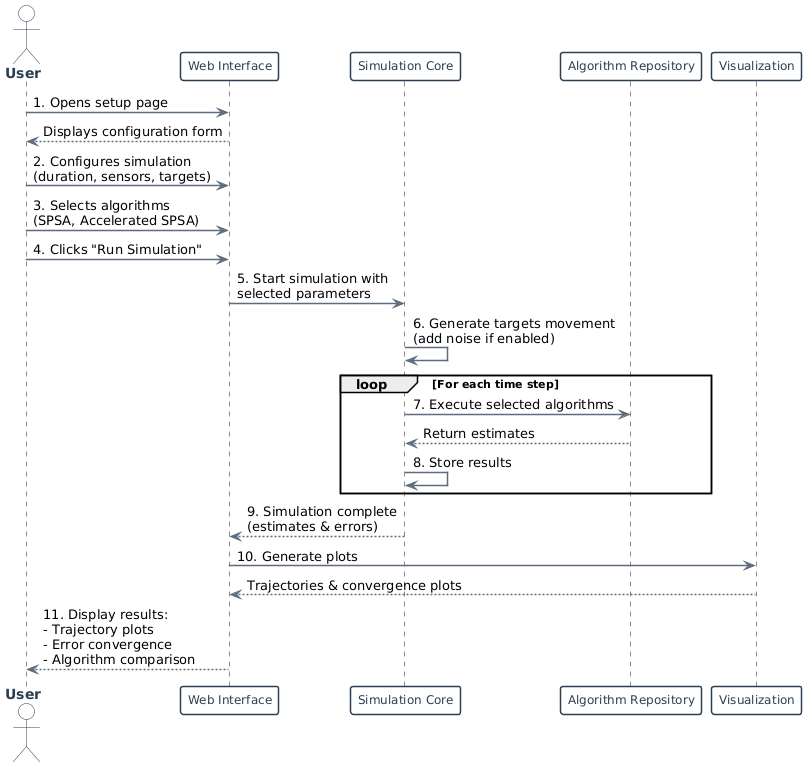
\includegraphics[width=0.95\textwidth]{use_case.png}
    \caption{Сценарий взаимодействия пользователя с системой}
    \label{fig:usecase}
\end{figure}

Сценарий работы пользователя включает следующие этапы:

\begin{enumerate}
    \item \textbf{Открытие страницы настройки.}  
    Пользователь переходит в веб-интерфейс и получает доступ к форме
    конфигурации.

    \item \textbf{Задание параметров симуляции.}  
    Пользователь задаёт длительность моделирования, количество целей и
    сенсоров, а также параметры шумов.

    \item \textbf{Выбор алгоритмов.}  
    Из репозитория выбираются алгоритмы для сравнения.

    \item \textbf{Запуск симуляции.}  
    Пользователь инициирует выполнение эксперимента.

    \item \textbf{Выполнение моделирования.}  
    Ядро моделирования выполняет расчёты, на каждом шаге времени
    вызывая выбранные алгоритмы.

    \item \textbf{Получение результатов.}  
    После завершения моделирования результаты передаются в систему
    визуализации.

    \item \textbf{Анализ результатов.}  
    Пользователь анализирует траектории, ошибки и сравнивает алгоритмы.
\end{enumerate}

Дополнительно система поддерживает пакетный режим, позволяющий
запускать серию экспериментов с последующим агрегированием результатов.

Таким образом, пользовательский сценарий (рис.~\ref{fig:usecase})
обеспечивает полный цикл работы с системой и соответствует
сформулированным требованиям.